\subsection{Entity Component System} % (fold)
\label{sub:Entity Component System}
TODO
% subsectionEntity Component System (end)

\subsubsection{ECS 是甚麼}
遊戲的本質其實就是大量物件(Entity)的行為以及它們之間的交互(Manager)。但顯然遊戲裡的物件不會只有少少幾個。隨著物件邏輯的增加,我們會將相同邏輯的部分進行拆分,由繁化簡,而拆分的方法有很多種。

\subsubsection{繼承}

最直接的寫法就是繼承,當我們的實體需要哪些邏輯的部分,我們就繼承那個部分。例如遊戲中地圖上有許多物品,這些物品(Item)分成裝飾和物件(Prop),裝飾是地圖上沒有物理、可以看見的實體;物件是可以互動、可以看見的實體;而地圖會有區域(Zone),切割地圖的區域和作為觸發(Trigger)使用。
所有的遊戲物件都繼承自 `GameObject` ,裏頭包含了位置等每個遊戲物體都有的資訊,`Zone` 內部實作碰撞,`Prop` 繼承自 `Zone` 實作了渲染,`Decoration` 也實作了渲染。可以發現到 `Prop` 跟 `Decoration` 只差在一個有碰撞,另一個沒有。如果我們嘗試將 `Prop` 改成繼承自 `Zone` 與 `Decoration` 則會導致菱形繼承,而這不是我們想要的。因此使用繼承並不能很好得解決這個問題。

\begin{figure}[h]
    \begin{center}
        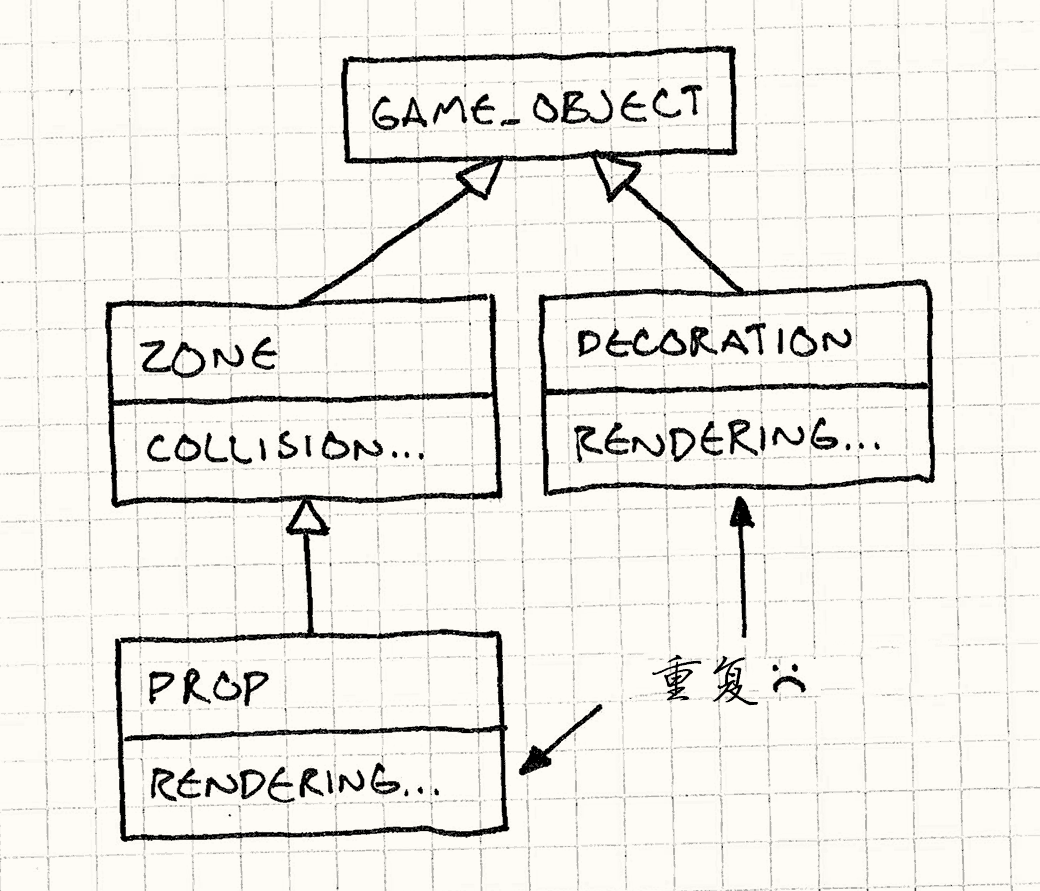
\includegraphics[width=0.5\textwidth]{./resources/ecs/inherit.png}
    \end{center}
\caption{繼承圖,取自 Game Programming Patterns}
\label{fig:inherit}
\end{figure}


\subsubsection{組件\(Component Pattern\)}

比起繼承,組件的靈活度更高。當我們需要那部分邏輯時,我們不再繼承他,而是讓物件擁有他。
這樣不但沒有宏偉的繼承樹,要讓各個實體溝通也就方便許多。

組件(Component)的優勢,讓我們只要將 Component 插入我們所要的對象,就能建構複雜且具有豐富行為的實體(Entity)。
由於單一個實體(Entity)跨越了多個領域(物理、渲染等等),為了保持領域之間的相互分離,將每部分的邏輯放進各自的組件(Component)。這意味著實體(Entity)被簡化成組件的容器。
簡單的`Component Pattern` 程式碼的遊戲流程會如下所示

\begin{lstlisting}
class Entity {

public:

    void update() {
    
        physis->update();
        transform->update();
        graphic->update();
    }

private:

    Physis* physis;
    Transform* transform;
    Graphic* graphic;
};

GameLoop() {

    while(running) {
    
        for(int i = 0 ; i < MAX_ENTITES ; i++)
            entityList->update();
    }
}
\end{lstlisting}

組件雖好,但這種方法對緩存不友好,CPU在抓取資料時會一次抓取一組資料進行處裡,稱為 `cache line`,每當CPU處理完當前任務,會先從 `cache line` 尋找下個任務,如果找到,就不再需要去記憶體裡面找下個任務。
我們的遊戲存取了每個實體的指標,而實體又儲存了每個組件的指標。每當要更新實體,我們得去遍歷他,又因為存取的是指標,因此會造成 `cache miss`,浪費寶貴的時間。每個實體又會更新每個組件,組件存的也是指標,又一次的`cache miss`。
一個遊戲注重的,除了遊戲本身好不好玩,另外一個就是效能了,`Entity Component System` 解決了這個問題。

\begin{figure}[h]
    \begin{center}
        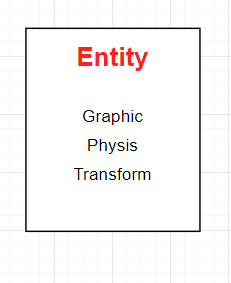
\includegraphics[width=0.5\textwidth]{./resources/ecs/componentPattern.png}
    \end{center}
\caption{組件圖}
\label{fig:component}
\end{figure}

\subsubsection{Entity Component System}

$Entity Component System$,簡稱$ECS$,這裡是指我們會有3個東西。$Entity$、 $Component$ 以及 $System$。

$ECS$ 與 $Component Pattern$ 不同的地方在於,$ECS$ 的 $Component$ 不再擁有任何的邏輯,$Component$ 所擁有的僅僅是 $Data$,而邏輯的部分全部移駕到對應的 $System$。這樣的好處是,$System$ 可以自己決定要操縱哪些$Data$。

\begin{itemize}
    \item{特徵}
        \SubItem{System 是唯一擁有邏輯的部分}
        \SubItem{Component 只擁有 Data}
        \SubItem{Entity 是多個 Component 的橋樑,用於表示這些 Component 是屬於這個 Entity 的。一般來說,Entity 僅僅只是一個 int}
    \item{好處} 
        \SubItem{由於 Data 被拆散了,不容易出現讀入整個對象卻只使用其中一個屬性的情況,有利於cache}
        \SubItem{狀態和邏輯分離,適合同步邏輯}
        \SubItem{所有同樣的 Component ,我們使用緊密的數組來儲存,因此我們能批量的連續進行處裡,這在理想的情況能夠大量減少 cache miss}
        \SubItem{由於 Component 只剩下 Data ,我們能夠很好的序列化}
\end{itemize}

\begin{figure}[h]
    \begin{center}
        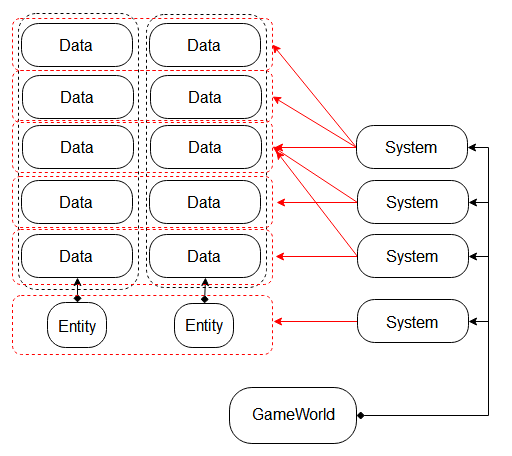
\includegraphics[width=0.5\textwidth]{./resources/ecs/ecs.png}
    \end{center}
\caption{ECS架構圖}
\label{fig:ecs}
\end{figure}

\subsubsection{實作}

\begin{itemize}
    \item{$ECS$ 將遊戲物件以及其行為拆成以下三樣東西}
        \SubItem{Entity}
        \SubItem{Component(Data)}
        \SubItem{System(Logic, behavior)}
\end{itemize}

\paragraph{Entity}

Entity僅是一個簡單的ID,他不會真的存著Component或任何其他東西,事實上他只會用來作為Component陣列的索引而已

\begin{lstlisting}
using Entity = std::uint32_t;
const Entity MAX_ENTITES = 10000;
\end{lstlisting}

\paragraph{Component}

Component只會存著需要的Data,不會擁有任何的邏輯

\begin{lstlisting}
struct Transform {

    vec3 position;
    vec3 size;
    float rotate;
};

struct Graphic {

    Texture texture_;
}
\end{lstlisting}

每種Component也會需要一個ID。

\begin{lstlisting}
using ComponentType = std::uint8_t;
const ComponentType MAX_COMPONENT = 32;
\end{lstlisting}

我們希望夠能追蹤這個Entity擁有哪些Component,同時也必須追蹤這個System會有哪些Component參與其中。

為了方便追蹤,我們會給Entity及System一個Signature,上面登記著它擁有了哪些Component。

std::bitset很適合達到我們的要求,前面我們幫每種Component訂了ID,意思是指要此物件或系統擁有這物件,就只要設定那個ID的bit。

舉個例子,Transform是0,Graphic是1,RigidBody是2,
擁有Transform和RigidBody的物件,它的Signature會被設定成0b101(bit 0, 2會被設定)。

\paragraph{Entity Manager}

Entity Manager是負責分配及追蹤Entity,記錄著哪些Entity ID已經被使用
用最簡單的std::queue就可以達成,當產生一個Entity,我們就返回一個Entity ID,當Entity被銷毀,我們再將此ID push回queue

\begin{lstlisting}
class EntityManager {

public:	

    Entity createEntity();
    void destroyEntity(Entity entity);
    void setSignature(Entity entity, Signature signature);
    Signature getSignature(Entity entity);

private: 

    // Array of signatures where the index is the Entity
    std::array<Signature, MAX_ENTITIES> Signatures_;
    // ALL Unused Entities
    std::queue<Entity> Entites_;
    // Total living Entites
    uint32_t EntitiesCounts_ = 0;
};

EntityManager::EntityManager() {
    // Unused Entites
    for(Entity entity = 0 ; entity < MAX_ENTITIES ; entity++)
        Entites_.push(entity);
}

Entity EntityManager::createEntity() {
    assert(EntitiesCounts_ < MAX_ENTITIES && "Too Many Entities");
    Entity id = Entites_.front();
    Entites_.pop();
    ++EntitiesCounts_;

    return id;
}

void EntityManager::destroyEntity(Entity entity) {
    assert(entity < MAX_ENTITIES && "Entity Out Of Range");
    Signatures_[entity].reset();
    Entites_.push(entity);
    --EntitiesCounts_;
}

void EntityManager::setSignature(Entity entity, Signature signature) {
    assert(entity < MAX_ENTITIES && "Entity Out Of Range");
    Signatures_[entity] = signature;
}

Signature EntityManager::getSignature(Entity entity) {
    assert(entity < MAX_ENTITIES && "Entity Out Of Range");
    return Signatures_[entity];
}
\end{lstlisting}



\paragraph{Component Array}
在這裡,我們必須實作一種簡單的陣列,但必須永遠是連續的,代表說它是不會有空洞出現的。
因為我們的Entity只是ID,要獲得跟Entity相關的Component是很簡單的,但是當Entity被銷毀時,對於陣列來說此Index(Entity ID)已經失效,我們不希望在遍歷陣列時出現失效的Entity。
但是事實上當Entity被銷毀時,它仍然是存在在陣列裡的。
在這裡,我們維護了兩個map,存著Entity ID與Index之間的關係。當要使用Entity時,利用Entity ID去尋找在陣列裡實際的位置。當Entity被移除時,我們將陣列裡最後一個尚未失效的Entity移動到被移除的位置上,接著只要更新map,一切就完成。
在這裡做個簡單的掩飾。

1. 我們假設MAX\_ENTITES 是 5,陣列一開始是空的,map也是空的

\begin{tabular}{@{} c|c|c|c|c|c|c @{}}
\headercell
Array & 0: & 1: & 2: & 3: & 4: & 5: \\
\midrule
Entity->Index &&&&&& \\
Index->Entity &&&&&& \\
Size & 0       &&&&& \\
\end{tabular}

2. 接著我們加入Entity A, 它的Entity ID為0,在陣列中的位置是0,所以將map的對應關係寫好

\begin{tabular}{@{} c|c|c|c|c|c|c @{}}
\headercell
Array & 0: & 1: & 2: & 3: & 4: & 5: \\
\midrule
Entity->Index & 0:0 &&&&& \\
Index->Entity & 0:0 &&&&& \\
Size & 1       &&&&& \\
\end{tabular}

3. 接著加入B

\begin{tabular}{@{} c|c|c|c|c|c|c @{}}
\headercell
Array & 0: & 1: & 2: & 3: & 4: & 5: \\
\midrule
Entity->Index & 0:0 & 1:1 &&&& \\
Index->Entity & 0:0 & 1:1 &&&& \\
Size & 2       &&&&& \\
\end{tabular}

4. 加入C

\begin{tabular}{@{} c|c|c|c|c|c|c @{}}
\headercell
Array & 0: & 1: & 2: & 3: & 4: & 5: \\
\midrule
Entity->Index & 0:0 & 1:1 & 2:2 &&& \\
Index->Entity & 0:0 & 1:1 & 2:2 &&& \\
Size & 3       &&&&& \\
\end{tabular}

5. 加入D -> 到這裡陣列保持連續,接著我們要刪除B,也就是Entity 1,為了保持連續,我們將D覆蓋B的位置然後更新map

\begin{tabular}{@{} c|c|c|c|c|c|c @{}}
\headercell
Array & 0: & 1: & 2: & 3: & 4: & 5: \\
\midrule
Entity->Index & 0:0 & 1:1 & 2:2 & 3:3 && \\
Index->Entity & 0:0 & 1:1 & 2:2 & 3:3 && \\
Size & 4       &&&&& \\
\end{tabular}

6. 刪除B

\begin{tabular}{@{} c|c|c|c|c|c|c @{}}
\headercell
Array & 0: & 1: & 2: & 3: & 4: & 5: \\
\midrule
Entity->Index & 0:0 & 3:1 & 2:2 &&& \\
Index->Entity & 0:0 & 1:3 & 2:2 &&& \\
Size & 3       &&&&& \\
\end{tabular}

7. 接著刪除Entity 3,也就是D

\begin{tabular}{@{} c|c|c|c|c|c|c @{}}
\headercell
Array & 0: & 1: & 2: & 3: & 4: & 5: \\
\midrule
Entity->Index & 0:0 & 2:1 &&&& \\
Index->Entity & 0:0 & 1:2 &&&& \\
Size & 2       &&&&& \\
\end{tabular}

8. 然後我們加入E,也就是Entity 4

\begin{tabular}{@{} c|c|c|c|c|c|c @{}}
\headercell
Array & 0: & 1: & 2: & 3: & 4: & 5: \\
\midrule
Entity->Index & 0:0 & 4:2 &&&& \\
Index->Entity & 0:0 & 2:4 &&&& \\
Size & 3       &&&&& \\
\end{tabular}

\begin{lstlisting}
class IComponentArray {

public:

    virtual ~IComponentArray() = default;
    virtual void entityDestroyed(Entity entity) = 0;
};

template<typename T>
class ComponentArray: public IComponentArray {

public:
    void insertData(Entity entity, T component) {

        assert(EntityToIndex.find(entity) == EntityToIndex.end() && "Components added to the same Entity more than once");
        size_t newIndex = size_;
        EntityToIndex[entity] = newIndex;
        IndexToEntity[newIndex] = entity;
        componentArray_[newIndex] = component;
        size_++;
    }

    void removeData(Entity entity) {

        assert(EntityToIndex.find(entity) != EntityToIndex.end() && "Entity does not exist");

        size_t remove = EntityToIndex[entity];
        size_t lastElement = size_-1;
        componentArray_[remove] = componentArray_[lastElement];
        Entity lastEntity = IndexToEntity[lastElement];
        EntityToIndex[lastEntity] = remove;
        IndexToEntity[remove] = lastEntity;
        EntityToIndex.erase(entity);
        IndexToEntity.erase(lastElement);
        size_--;
    }

    T& getComponent(Entity entity) {

        assert(EntityToIndex.find(entity) != EntityToIndex.end() && "retrieving none exist component");
        return componentArray_[EntityToIndex[entity]];
    }

    void entityDestroyed(Entity entity) override {

        if(EntityToIndex.find(entity) != EntityToIndex.end())
            removeData(entity);
    }

private:

    std::array<T, MAX_ENTITIES> componentArray_;
    std::unordered_map<Entity, size_t> EntityToIndex;
    std::unordered_map<size_t, Entity> IndexToEntity;
    size_t size_ = 0;
};
\end{lstlisting}

\footnote{這層抽象層是必要的,我們會有很多的Component array,並且用一個list存著他們,每當有Entity被銷毀時,我們必須逐一地去通知他們有Entity被銷毀了。能讓我們存各個不同type的Component的辦法就是有一層抽象層了。}

\paragraph{Component Manager}

Component Manager是負責管理所有的Component Array的,並不是讓他們之間溝通,而是通知他們我註冊了哪些Component,或是該刪除哪些Component

\begin{lstlisting}
class ComponentManager {

public:
    template<typename T>
    void registerComponent() {

        const char* typeName = typeid(T).name();
        assert(componentTypes_.find(typeName) == componentTypes_.end() && "Registering component type more than once");
        componentTypes_.insert({typeName, nextComponentType_});
        componentArray_.insert({typeName, std::make_shared<ComponentArray<T>>()});
        ++nextComponentType_;
    }

    template<typename T>
    ComponentType getComponentType() {

        const char* typeName = typeid(T).name();
        assert(componentTypes_.find(typeName) != componentTypes_.end() && "Component did not register");
        return componentTypes_[typeName];
    }

    template<typename T>
    void addComponent(Entity entity, T component) {

        getComponentArray<T>()->insertData(entity, component);
    }

    template<typename T>
    void removeComponent(Entity entity) {

        getComponentArray<T>()->removeData(entity);
    }

    template<typename T>
    T& getComponent(Entity entity) {

        return getComponentArray<T>()->getComponent(entity);
    }

    void entityDestroyed(Entity entity) {

        for(auto const& pair: componentArray_) {

            auto const& component = pair.second;
            component->entityDestroyed(entity);
        }
    }


private:

    std::unordered_map<const char*, ComponentType> componentTypes_;
    std::unordered_map<const char*, std::shared_ptr<IComponentArray>> componentArray_;
    ComponentType nextComponentType_ = 0;

    template<typename T>
    std::shared_ptr<ComponentArray<T>> getComponentArray() {

        const char* typeName = typeid(T).name();
        assert(componentTypes_.find(typeName) != componentTypes_.end() && "Component did not register");

        return std::static_pointer_cast<ComponentArray<T>>(componentArray_[typeName]);
    }
};
\end{lstlisting}


\subsubsection{System}

System是行為存在的地方。
每個System都放著存著Entity的list


\begin{lstlisting}
class System {

public:
    std::set<Entity> Entities_;
};
\end{lstlisting}

當我們需要實作系統就時繼承它

\begin{lstlisting}
class PhysicSystem : public System {

public:

    void update(float dt);

};

class GraphicSystem : public System {

public:

    void update();
    
    void render(sf::RenderTarget& target);
};
\end{lstlisting}

而System的更新方法,會將此系統所在乎的Component(Data),取出,並進行更新。

\begin{lstlisting}
void PhysicSystem::update(float dt) {

    for(auto const& entity : Entities_) {

        auto& transform = ecs.getComponent<Transform>(entity);
        auto& rigidBody = ecs.getComponent<RigidBody>(entity);

        transform.y_ += rigidBody.v_ * dt;

        rigidBody.v_ +=  10 * dt;
    }
}
\end{lstlisting}

/footnote{物理系統關心實體的Transform以及RigidBody,因此沒有這兩個 Component的實體,系統是不會去更新他們。}


\paragraph{System Manager}

System Manager是負責管理所有的System及他們的Signature。
每個System的Signature代表此System會用到的Component,以便將合適的Entity分配給它。
當Entity被銷毀,System的list也得跟著更新。

\begin{lstlisting}
class SystemManager {

public:
    template<typename T>
    std::shared_ptr<T> registerSystem() {

        const char* typeName = typeid(T).name();
        assert(system_.find(typeName) == system_.end() && "Registering system more than once");
        auto system = std::make_shared<T>();
        system_.insert({typeName, system});
        return system;
    }

    template<typename T>
    void setSignature(Signature signature) {

        const char* typeName = typeid(T).name();
        assert(system_.find(typeName) != system_.end() && "System did not register");
        signatures_.insert({typeName, signature});
    }

    void entityDestroyed(Entity entity) {

        for(auto const& pair : system_) {

            auto const& system = pair.second;
            system->Entities_.erase(entity);
        }
    }

    void entitySignatureChanged(Entity entity, Signature entitySignature) {

        for(auto const& pair: system_){

            auto const& type = pair.first;
            auto const& system = pair.second;
            auto const& systemSignature = signatures_[type];

            if((entitySignature & systemSignature) == systemSignature) system->Entities_.insert(entity);
            else system->Entities_.erase(entity);
        }
    }

private:

    std::unordered_map<const char*, Signature> signatures_;
    std::unordered_map<const char*, std::shared_ptr<System>> system_; 
};
\end{lstlisting}

\paragraph{ECS}

擁有管理Entity的Entity Manager、管理Component的Component Manager以及管理System的System Manager之後,最後就是將三個Manager封裝起來。

\begin{lstlisting}
class ECS {

public:

    ECS() = default;
    void init();
    Entity createEntity();
    void destroyEntity(Entity entity);
    template<typename T>
    void registerComponent() {

        componentManager_->registerComponent<T>();
    }

    template<typename T>
    void addComponent(Entity entity, T component) {

        componentManager_ ->addComponent<T>(entity, component);
        auto signature = entityManager_->getSignature(entity);
        signature.set(componentManager_->getComponentType<T>(), true);
        entityManager_->setSignature(entity, signature);

        systemManager_->entitySignatureChanged(entity, signature);
    }

    template<typename T>
    void removeComponent(Entity entity){

        componentManager_->removeComponent<T>(entity);
        auto signature = entityManager_->getSignature(entity);
        signature.set(componentManager_->getComponentType<T>(), false);
        entityManager_->setSignature(entity, signature);
        systemManager_->entitySignatureChanged(entity, signature);
    }

    template<typename T>
    T& getComponent(Entity entity) {

        return componentManager_->getComponent<T>(entity);
    }

    template<typename T>
    ComponentType getComponentType() {

        return componentManager_->getComponentType<T>();
    }

    template<typename T>
    std::shared_ptr<T> registerSystem() {

        return systemManager_->registerSystem<T>();
    }

    template<typename T>
    void setSystemSignature(Signature signature) {

        systemManager_->setSignature<T>(signature);
    }

private:

    std::unique_ptr<EntityManager> entityManager_;
    std::unique_ptr<ComponentManager> componentManager_;
    std::unique_ptr<SystemManager> systemManager_;
};


void ECS::init() {

    entityManager_ = std::make_unique<EntityManager>();
    componentManager_ = std::make_unique<ComponentManager>();
    systemManager_ = std::make_unique<SystemManager>();
}


Entity ECS::createEntity() {

    return entityManager_->createEntity();
}

void ECS::destroyEntity(Entity entity) {

    entityManager_->destroyEntity(entity);
    componentManager_->entityDestroyed(entity);
    systemManager_->entityDestroyed(entity);
}

\end{lstlisting}

\paragraph{使用方法,假設擁有有三個Component}

\begin{lstlisting}
struct Transform{

public:
    float x_;
    float y_;
};


struct RigidBody{

public:
    float v_;
};

struct Graphic{

public:

    Texture texture;
};
\end{lstlisting}

\paragraph{我們的Graphic System}

\begin{lstlisting}
class GraphicSystem : public System {

public:

    void render(RenderTarget& target);
};


void GraphicSystem::render() {

    for(auto const& entity : Entities_) {

        auto& graphic = ecs.getComponent<Graphic>(entity);
        auto& transform = ecs.getComponent<Transform>(entity);
        
        Renderer::Draw(transform.x, transform.y, graphic.texture);
    }
}
\end{lstlisting}

\paragraph{PhysicSystem}

\begin{lstlisting}
class PhysicSystem : public System {

public:

    void update(float dt);

};

void PhysicSystem::update(float dt) {

    for(auto const& entity : Entities_) {

        auto& transform = ecs.getComponent<Transform>(entity);
        auto& rigidBody = ecs.getComponent<RigidBody>(entity);

        transform.y_ += rigidBody.v_ * dt;

        rigidBody.v_ +=  10 * dt;
    }
}
\end{lstlisting}


\paragraph{初始化}

\begin{lstlisting}
ECS::ECS ecs;

ecs.init();
ecs.registerComponent<ECS::Transform>();
ecs.registerComponent<ECS::RigidBody>();
ecs.registerComponent<ECS::Graphic>();
\end{lstlisting}

\paragraph{註冊System以及設定signature}

\begin{lstlisting}
auto graphicSystem = ecs.registerSystem<ECS::GraphicSystem>();
ECS::Signature signature;
signature.set(ecs.getComponentType<ECS::Graphic>());
signature.set(ecs.getComponentType<ECS::Transform>());
ecs.setSystemSignature<ECS::GraphicSystem>(signature);

auto physicSystem = ecs.registerSystem<ECS::PhysicSystem>();
signature.set(ecs.getComponentType<ECS::Transform>());
signature.set(ecs.getComponentType<ECS::RigidBody>());
ecs.setSystemSignature<ECS::PhysicSystem>(signature);
\end{lstlisting}

\paragraph{產生Entity}

\begin{lstlisting}
std::vector<ECS::Entity> entites(ECS::MAX_ENTITIES);

for(auto& entity: entites) {

    entity = ecs.createEntity();
    ecs.addComponent(
        entity,
        ECS::Transform{randPositionX(generator), randPositionY(generator), p}
    );
    ecs.addComponent(
        entity,
        ECS::RigidBody{20}
    );
    ecs.addComponent(
        entity,
        ECS::Graphic{texture}
    );
}
\end{lstlisting}

\newpage